
\section{Microgrids}\label{microgrids}
%We hebben afgesproken dat we de boel even wat gaan omschoppen opdat het hoofdstuk zich meer zal richten op game theory. Voorstel: 
%4.1 Grouping of DER
%4.2 Game of perfect information
%4.3 Stored energy management
%--- Vervolgens aantal subsub sections


Another challenge in de design of Smart Grids is managing energy generation and storage. This challenge is impacted by geographical limitations, as energy loss has a big \todo{invloedhebber} impact when transferring energy.\cite{EnergyLossURL}
Microgrids can solve this problem by managing all supply and demand within a geographical area. When introducing microgids, new challenges arise: In what way should microgrids communicate with eachother? but also creates the opportunity to utilize game theoretic methods to compute local nash equilibria, such as a Dynamic Game of Perfect information and a Double Auction Game.
Microgrids can operate in both isolation(islanded mode) as in conjunction with the smart grid\ref{HatziargyriouAsanoIravaniMarnay2007}. 
A example model of a neighbourhood microgrid can be seen in figure \ref{img:microgrid-model}


%Other challenges in the design of Smart Grids are  the complexity of calculating equilibria and managing energy generation and storage. Constructing microgrids, in essence a geographical limited smart grid, gives us the opportunity to utelise Game Theoretic methods such as a Game of Perfect information and double auction game. 
%Current electrical grids actually already do this: neighbourhood homes are connected to a central distribution point, which connects to the main grid.
%Microgrids can solve, or optimise, challenges in smart-grids which are too large to tackle or too complex to solve. The concept of Microgrids can also help with the Stored energy management.



\subsection{Complexity}

As discussed in chapter two, calculating nash equilibria is almost as hard as calculating NP-hard problems. When making algorithms approximating the nash equilibria, heuristics are definitely needed. Smart-grids have a lot of players and microgrids reduce this number drastically. Therefore, computing an approximation for nash equilibrium will cost relatively less computing power.


\paragraph{Game of perfect information}
When having a microgrid as modelled in figure \ref{img:microgrid-model}, we can use a Game Theoretic Approach called a "dynamic game of perfect information" to calculate a nash equilibriumAll local Controllers (Smart Agents in the homes and for each \acr{DER}

When using microgrids, the game of perfect information can be used to create an equilibrium in microgrids. Because the number of players is limited in a microgrid, both for the demand side as well as the supply side, it is less complex and time consuming to calculate the best options considering each players' wishes. Then, a price can be determined by a Aggregator, who can decide whether to buy or sell electricity for the whole microgrid. The aggregator is modelled as a Smart Agent\cite{MicrogridModellingPetrosAristidou}.

The Microgrid model can be examined under the class of games called ”Dynamic

Games of Perfect Information”. Dynamic games are games with sequential move

order, meaning, some players move or act only after having observed someone

else’s move or action. Perfect Information denotes that at every round of the

game, the player whose turn is to chose an action knows the actions other play-
ers have chosen before him. The game formed by the Microgrid model can be

of complete information, meaning that every players revenue function is com-
mon knowledge, or incomplete information [6]. We can see the extensive form

representation of the game in 2.

\begin{figure}
	\caption{Microgrid model}
	\centering
	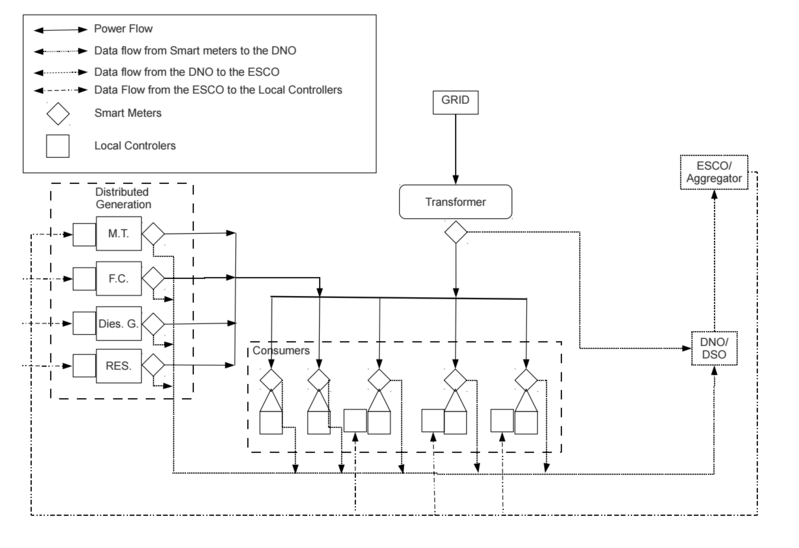
\includegraphics[width=1\linewidth]{images/game-of-perfect-information.png}
	\label{img:microgrid-model}
\end{figure}

\subsection{Energy management}
\todo{Talk about energy management in general, how microgrids can improve and something about the physical distance}
In microgrids heb je minder players 
As you have read before, microgrids can help in reducing energy loss. The loss of energy is caused mainly by two factors \cite{EnergyLossURL}: 

\begin{enumerate}
\item Energy transmission from power plants to local distributors is done trough power lines, which suffer from losses due to i.e. heat generation\cite{LasseterPaigi2004}.
\item In an energy grid, each transformer has a certain efficiency, which is never 100\%. Reducing the number of transformers will reduce overall energy loss.
\end{enumerate}

Microgrids will be able to reduce energy loss because within microgrids generated power can be used for local demand and can communicate with other nearby microgrids. It can also help to avoid the power losses found in a substation's transformer \cite{keypaper}.

Whenever some microgrids have an excess of power while others have a need for power, it might be beneficial for these microgrids (and their consumers) to exchange energy among each other instead of requesting it from the main grid \cite{SaadHanPoorEtAl2011}. To manage this, the same cooperative game theory concepts as discussed in \ref{microgrids:cooperation} can be used. When the power loss of a trade is mapped to the value of the corresponding coalition, that power loss can be minimised, contributing to the efficiency of the entire smart grid. 

The buying and selling of energy between microgrids can be guided by another cooperative game theory using auctions, as proposed in \cite{SaadHanPoorEtAl2011}. This involves matching several buyers and sellers within one or more coalition and agreeing on some price. This price $p$ can be obtained through the use of a \emph{double auction}, where all sellers asking $p$ or less and all buyers offering $p$ or more are matched and trade using $p$ \cite{gjerstad1998price}.

\subsubsection{\ac{ev} groups}
The growing usage of \ac{ev}s offers a lot of possibilities for microgrids because it expands the storage capacity of a microgrid tremendously. One of the key challenges in integrating \ac{ev}s in a smart grid is modelling the interactions of all actors. In \cite{SaadHanPoorEtAl2011} a noncooperative game is formulated between \ac{ev} groups where groups strategically choose how much of their energy surplus is sold. A double auction based mechanism is given to determine the energy price of the energy trade market, to assure a strategy-proof outcome. 



% Goede papers:
%	http://ieeexplore.ieee.org/stamp/stamp.jsp?arnumber=5546904
% ,HatziargyriouAsanoIravaniMarnay2007
% MicrogridModellingPetrosAristidou

